\subsubsection{Data Description and Preprocessing}
\textit{ATAC-seq} is an emerging evoluted technique which enables to investigate the open chromatin regions at whole genome level.
The capability of this technology has been demonstrated in the regulation of mouse brain activity under different conditions \cite{Su2017}.

To illustrate the performances of \gls{descan} we chose a dataset \cite{Su2017} that describes in vivo adult mouse dentate granule neurons before and after synchronous neuronal activation using \textit{ATAC-seq} and \textit{RNA-seq} technologies (see sections \ref{sec:atacseq} and \ref{sec:rnaseq} for a description of these sequencing techniques).

This dataset is organized in 62 samples of \textit{ATAC-seq} and \textit{RNA-seq}, extracted at four different time points (0, 1h, 4h, 24h), with four replicates at each time point.
We chose to compare the differences between the first two stages, time 0 (E0) and 1 hour after neuronal induction (E1), in order to show a potential \textit{ATAC-seq} workflow for Differential Enrichment, and how to integrate this data type with \textit{RNA-seq}. A general illustration of this dataset is represented in figure \ref{fig:atacdataset}.

\begin{figure}[H]
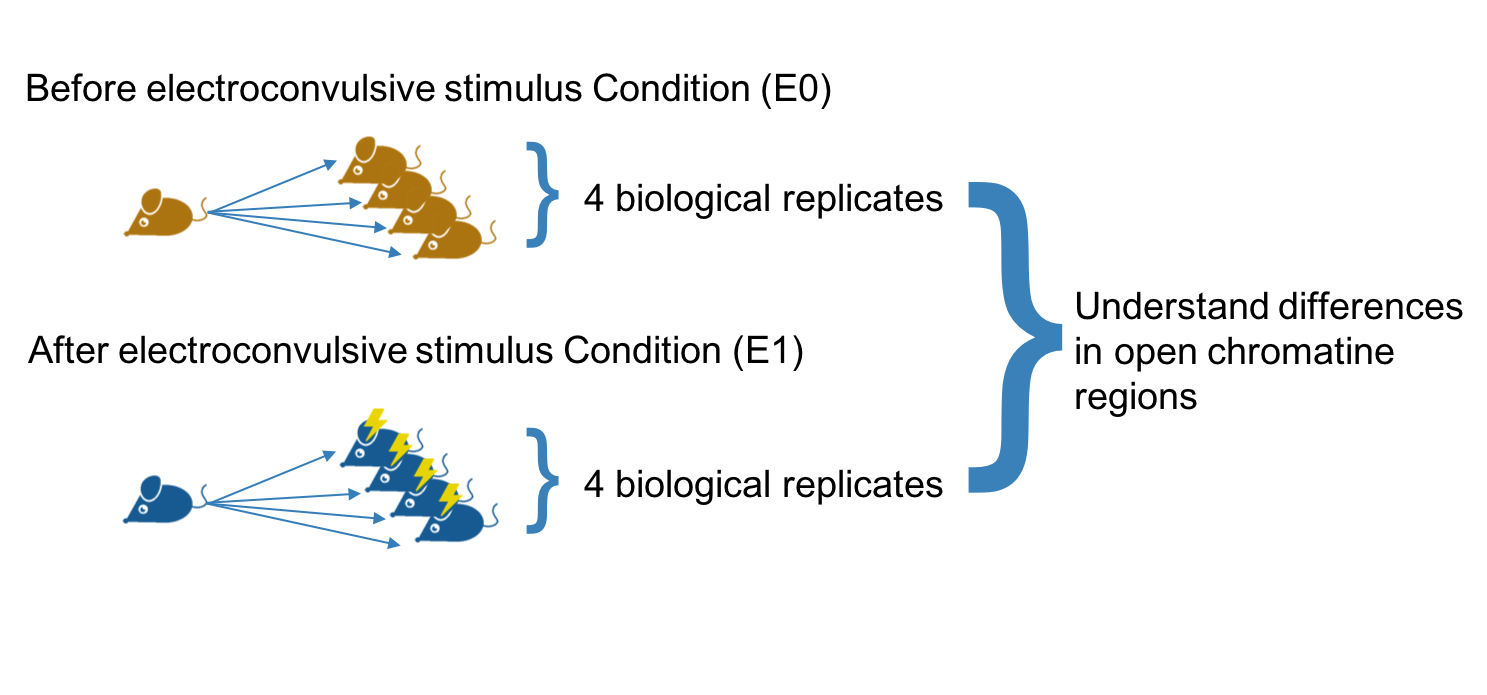
\includegraphics[width=\textwidth, keepaspectratio]{img/descan2/dataset.png}
\caption[DEScan2 dataset illustration]{An illustration of our extraction of the GSE82015\cite{Su2017} dataset.}
\label{fig:atacdataset}
\centering
\end{figure}

We downloaded the data from \gls{geo} database \cite{Edgar2002, Barrett2013} with accession number GSE82015\footnote{\url{https://www.ncbi.nlm.nih.gov/geo/query/acc.cgi?acc=GSE82015}} and mapped the raw data using \textit{STAR} \cite{Dobin2013} with default parameter on \gls{mm10}.

\subsubsection{Peaks Detection}

In order to detect open chromatin regions, we run our peak caller, cutting the genome in bins of 50bp and using running windows of minimum 50bp and maximum 1000bp.
In this way, we are able to detect not just broad peaks, but also smaller peaks.

To be confident with our results we run \gls{descan} and \textit{MACS2}  \cite{Zhang2008} on the same samples, and (as shown in figure \ref{fig:des2m2peaks}) looking to the numbers \gls{descan} always find more peaks than \textit{MACS2}.
This can be due to a major accuracy gave by \textit{MACS2} on the reliability of the detected peaks, while our method finds more peaks, but, at this stage, still preserving false positive regions.

\begin{figure}[H]
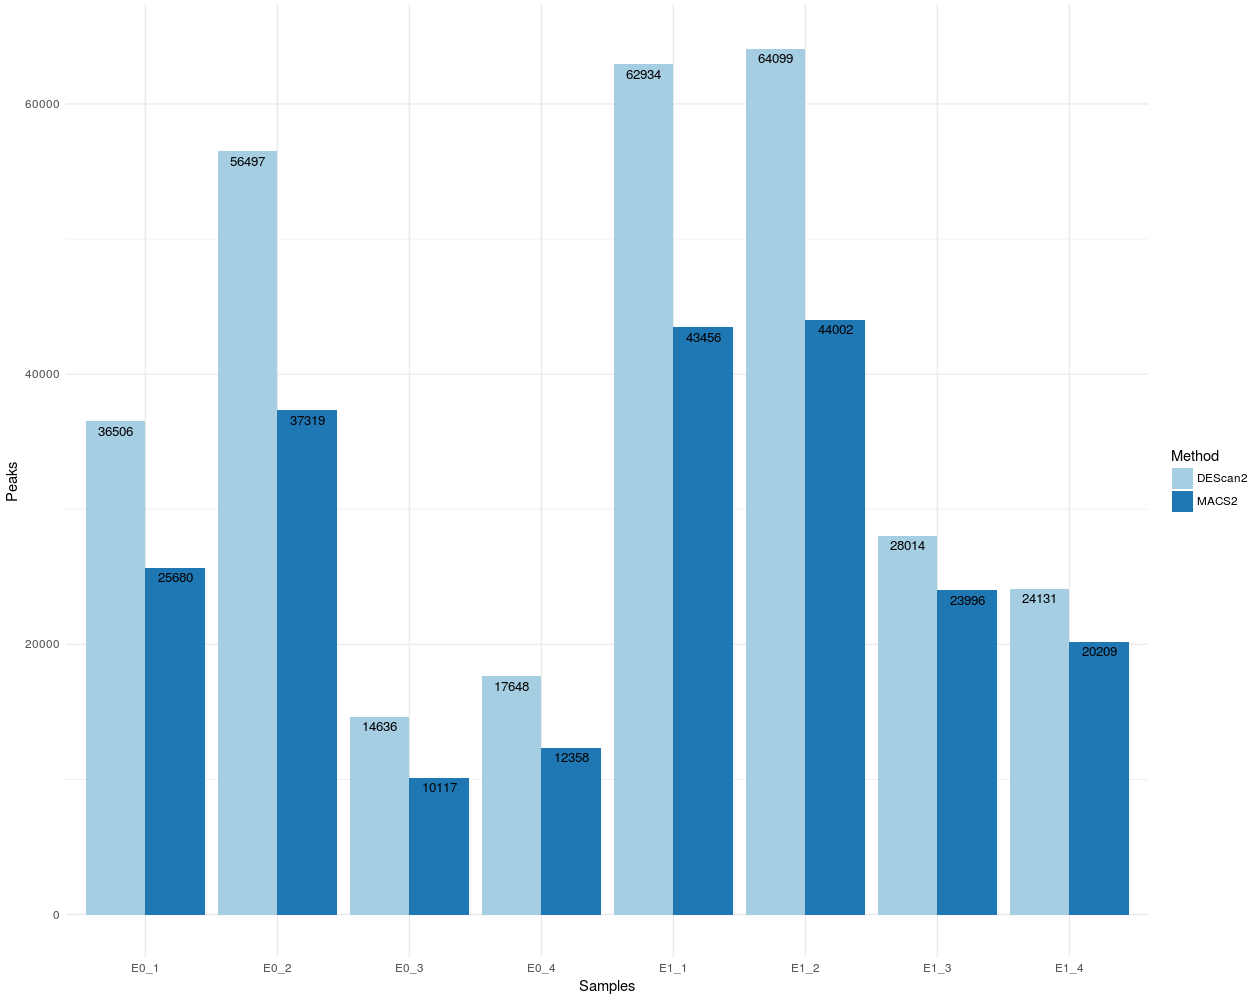
\includegraphics[width=\textwidth, keepaspectratio]{img/descan2/d2m2_peaks_number.png}
\caption[The \gls{descan} and \textit{MACS2} peaks detection]{A comparison of \gls{descan} and \textit{MACS2} detected peaks for each sample in the dataset.}
\label{fig:des2m2peaks}
\centering
\end{figure}

To be more robust, we compared \gls{descan} detected peaks with the same validated regions (\textit{Arc}\footnote{https://www.genecards.org/cgi-bin/carddisp.pl?gene=ARC} and \textit{Gabrr1}\footnote{https://www.genecards.org/cgi-bin/carddisp.pl?gene=GABRR1}) of the original work \cite{Su2017}.
The lower part of figure \ref{fig:peaksdescan} shows the detected and validated regions (in blue and red) resulting differentially enriched between the E0 (in pink) and E1 (in green) conditions, while the upper part shows \gls{descan} filtered and aligned peaks (in blue) between the samples, highlighting a capability to catch not only the same regions of the published ones but also (gold circles) to be more accurate in the smaller peaks detection.

\begin{figure}[H]
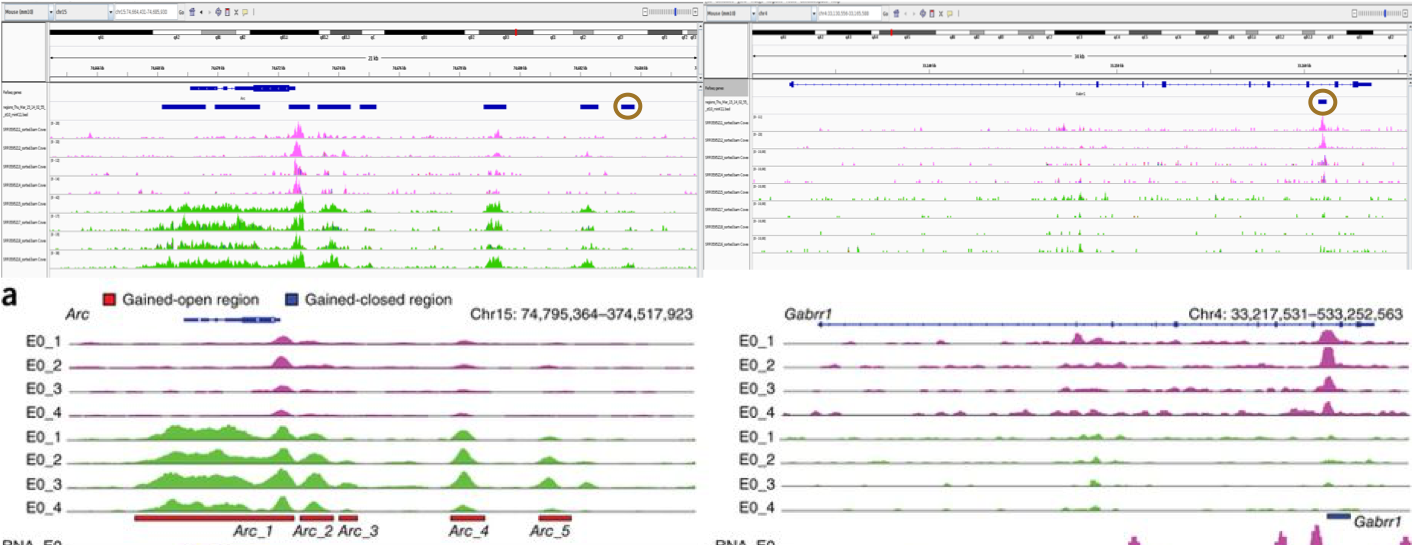
\includegraphics[width=\textwidth, keepaspectratio]{img/descan2/peaks.png}
\caption[\gls{descan} peaks detection]{A comparison of \gls{descan} detected peaks with validated peaks in article \cite{Su2017}.}
\label{fig:peaksdescan}
\centering
\end{figure}

\subsubsection{Removing Unwanted Peaks}

While it is very important to detect good peaks with a peak caller, it seems to be more relevant to detect reproducible regions. 
Indeed, during the filtering/aligning step, the number of peaks depends not only by the peak score but also by the number of replicates designed in the experiment.
The figure \ref{fig:filteringdescanmacs2} puts in relation these two relevant information for both \textit{MACS2} and \gls{descan}. 
On the x-axis is represented the number of replicates, while on the y-axis is traced the number of peaks, and each curve represents a different threshold on the peaks score, showing that the higher is the thresholds on the scores and the number of replicates, the lower is the number of the detected peaks.
Highlighting a inverse relationship between the number of the peaks and the combination of the number of samples and the detected regions score.
%\begin{figure}[H]
%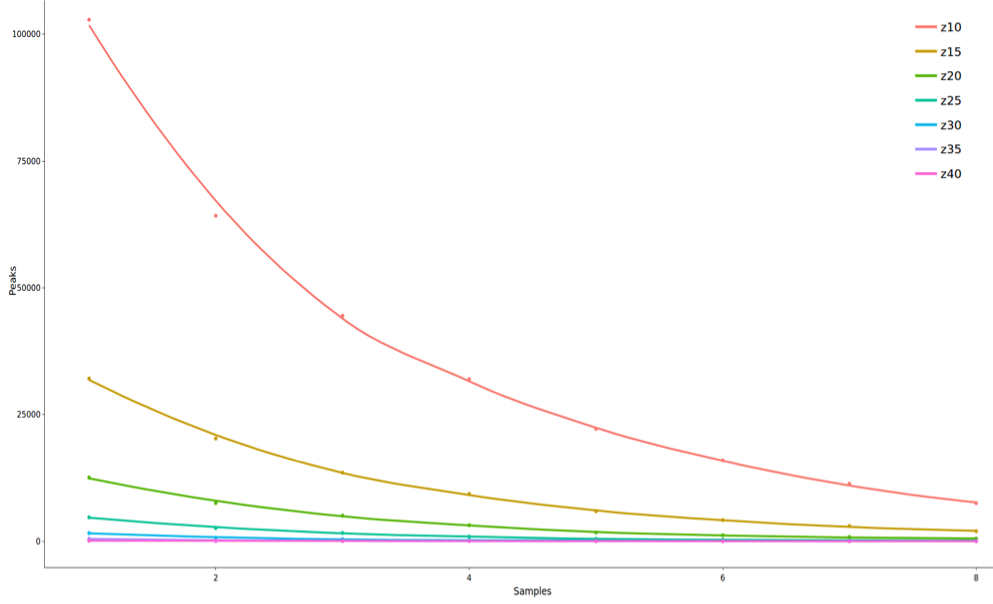
\includegraphics[width=\textwidth, height=\textheight, keepaspectratio]{img/descan2/filtering.png}
%\caption[\gls{descan} filtering step]{Filtering the detected regions with different thresholds on peak scores.}
%\label{fig:filteringdescan}
%\centering
%\end{figure}

\begin{figure}[H]
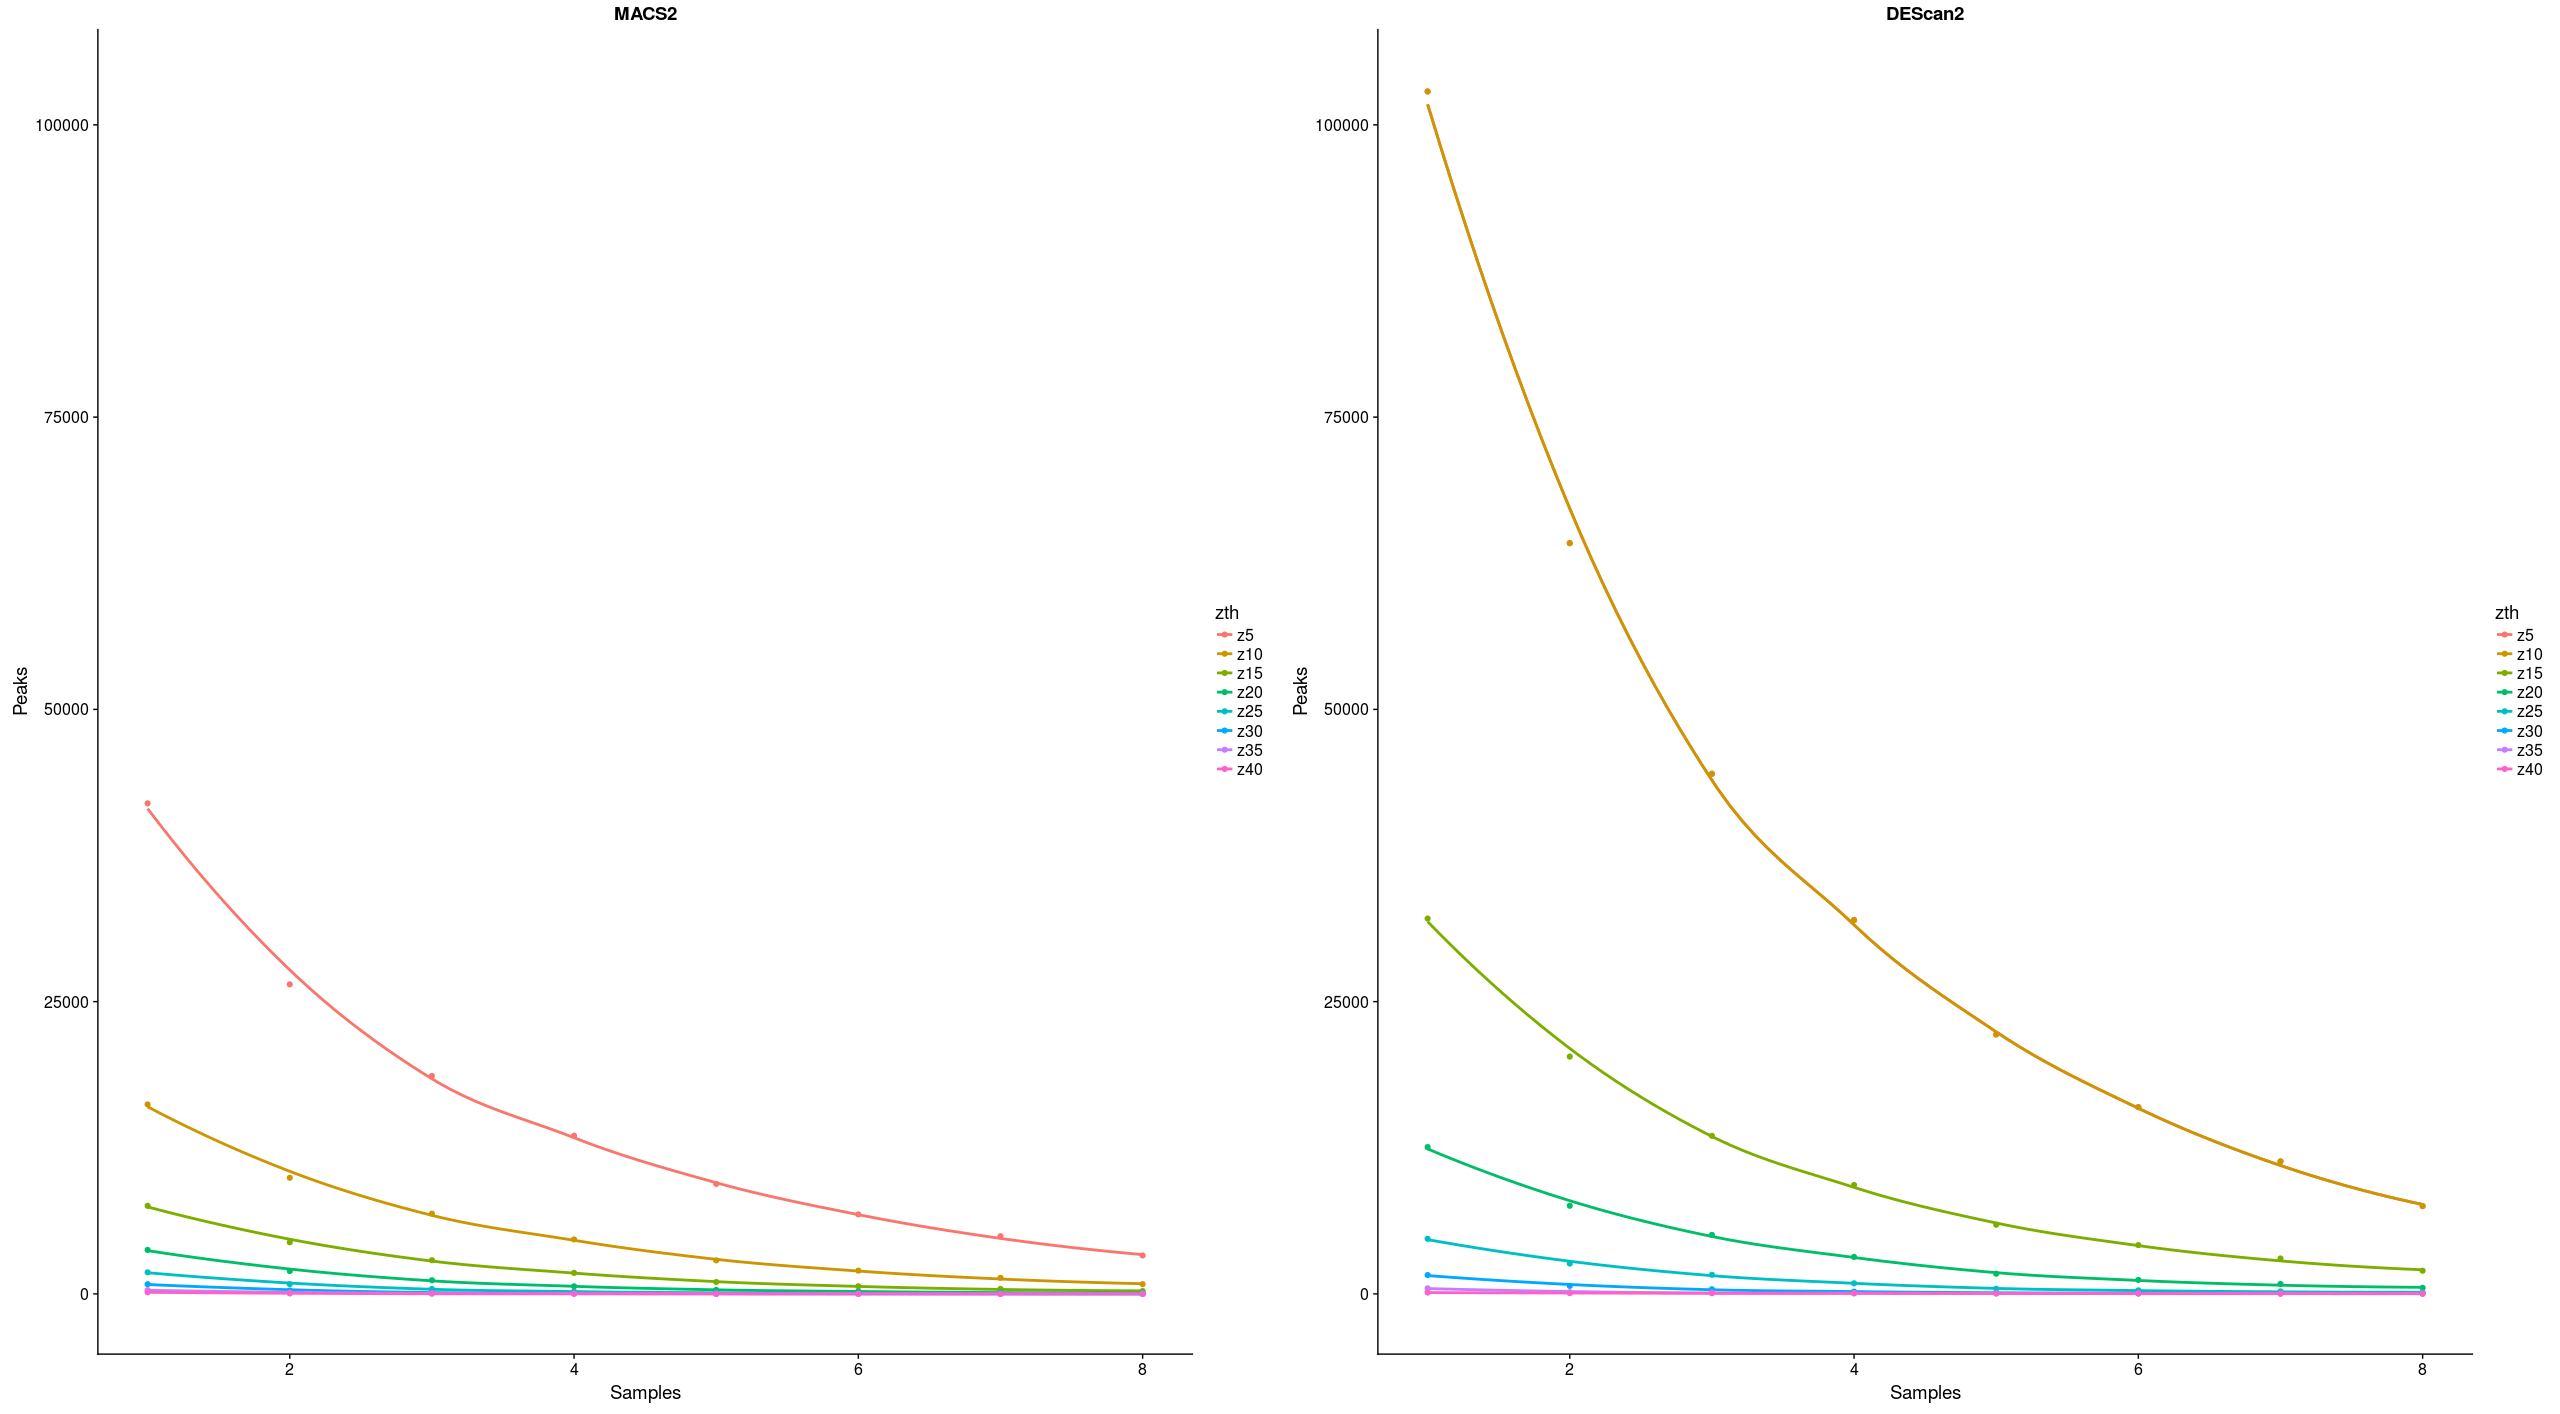
\includegraphics[width=\textwidth, keepaspectratio]{img/descan2/filtering_m2_d2.png}
\caption[\gls{descan} and \textit{MACS2} filtering comparison]{Filtering the detected regions with different thresholds on peak scores between \textit{MACS2} and \gls{descan}.}
\label{fig:filteringdescanmacs2}
\centering
\end{figure}


Moreover, comparing the left and right panels, we notice the high difference in pooling the samples-peaks together with the \gls{descan} filtering/aligning step when using \textit{MACS2} and \gls{descan} peaks.
Using \textit{MACS2} peaks the pooling highly reduces the number of detected peaks, even using a threshold as low as 5 on the score, showing that there are many peaks with a score lower than 5.
While in the \gls{descan} case the curves representing the threshold equal to 5 and the threshold equal to 10 totally overlap, highlighting that the \gls{descan} peak caller produces scores higher than 10.

%\textbf{MAGARI QUESTO CONFRONTO è DA EVITARE NON FILTRANDO CON IL NOSTRO METODO I PICCHI DI MACS2, NON SO!}

\subsubsection{Quantifying Peaks}

Afterwards, the filtered-in regions can be processed by \gls{descan} in order to obtain a count matrix with samples on the columns and peaks on the rows.
This type of data structure is very versatile because it enables to perform several operations, like the \glspl{der} and the integration with other kinds of omics, as \textit{RNA-seq}.

\begin{figure}[H]
\centering
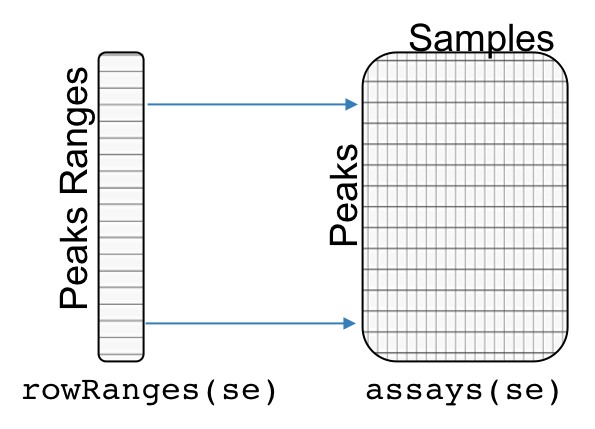
\includegraphics[scale=.7]{img/descan2/counts.png}
\caption[\gls{descan} counts illustration]{An illustration of the \textit{SummarizedExperiment} data structure produced by \gls{descan}.}
\label{fig:countsdescan}
\centering
\end{figure}

In order to preserve the information associated to the peaks, \gls{descan} produces as output a \textit{SummarizedExperiment} (figure \ref{fig:countsdescan}) data structure, which enables to retrieve the count matrix with \lstinline!assays! method, and to access the peaks information in \textit{GenomicRanges} format with the \lstinline!rowRanges! method.


\subsubsection{Peaks Normalization}

Before detecting \glspl{der}, it is a good practice to normalize the data.
This is especially needed when working with neuroscience data, where many possible sources of technical and biological noise can confound the analysis \cite{Peixoto2015}.
The nature of the data, in count format, makes it possible to apply several well known RNA-Seq normalizations techniques, such as \textit{upper-quartile}, \textit{full-quantile}, \textit{RUV-Seq}, etc \cite{Risso2014h, Dillies2013}.
To filter out false positives, but preserving enough signal at the same time, we fixed the peaks score threshold to 20.

In order to compare the effects of normalizations we had to do differential enrichment of the conditions using \textit{edgeR} (see next section for further details).

While the \textit{upper-quartile} normalization affects the data in a way that makes it impossible to detect \glspl{der}, other kinds of normalizations and combinations of them give good results.

Figure \ref{fig:normalizationsfull} summarizes this concept very well, highlighting a relation between the number of \glspl{der} (y-axis) and the minumum number of samples (x-axis) used for aligning the peaks during the \gls{descan} filtering/aligning step.

To better compare the normalization effects, we created a \textit{null dataset} of 8 samples, by shuffling the original dataset samples as combinations of conditions took in pairs.
The detection of \glspl{der} has been performed on each combination ($18$) of shuffled samples and then taking the median of the results.

\begin{figure}[H]
\centering
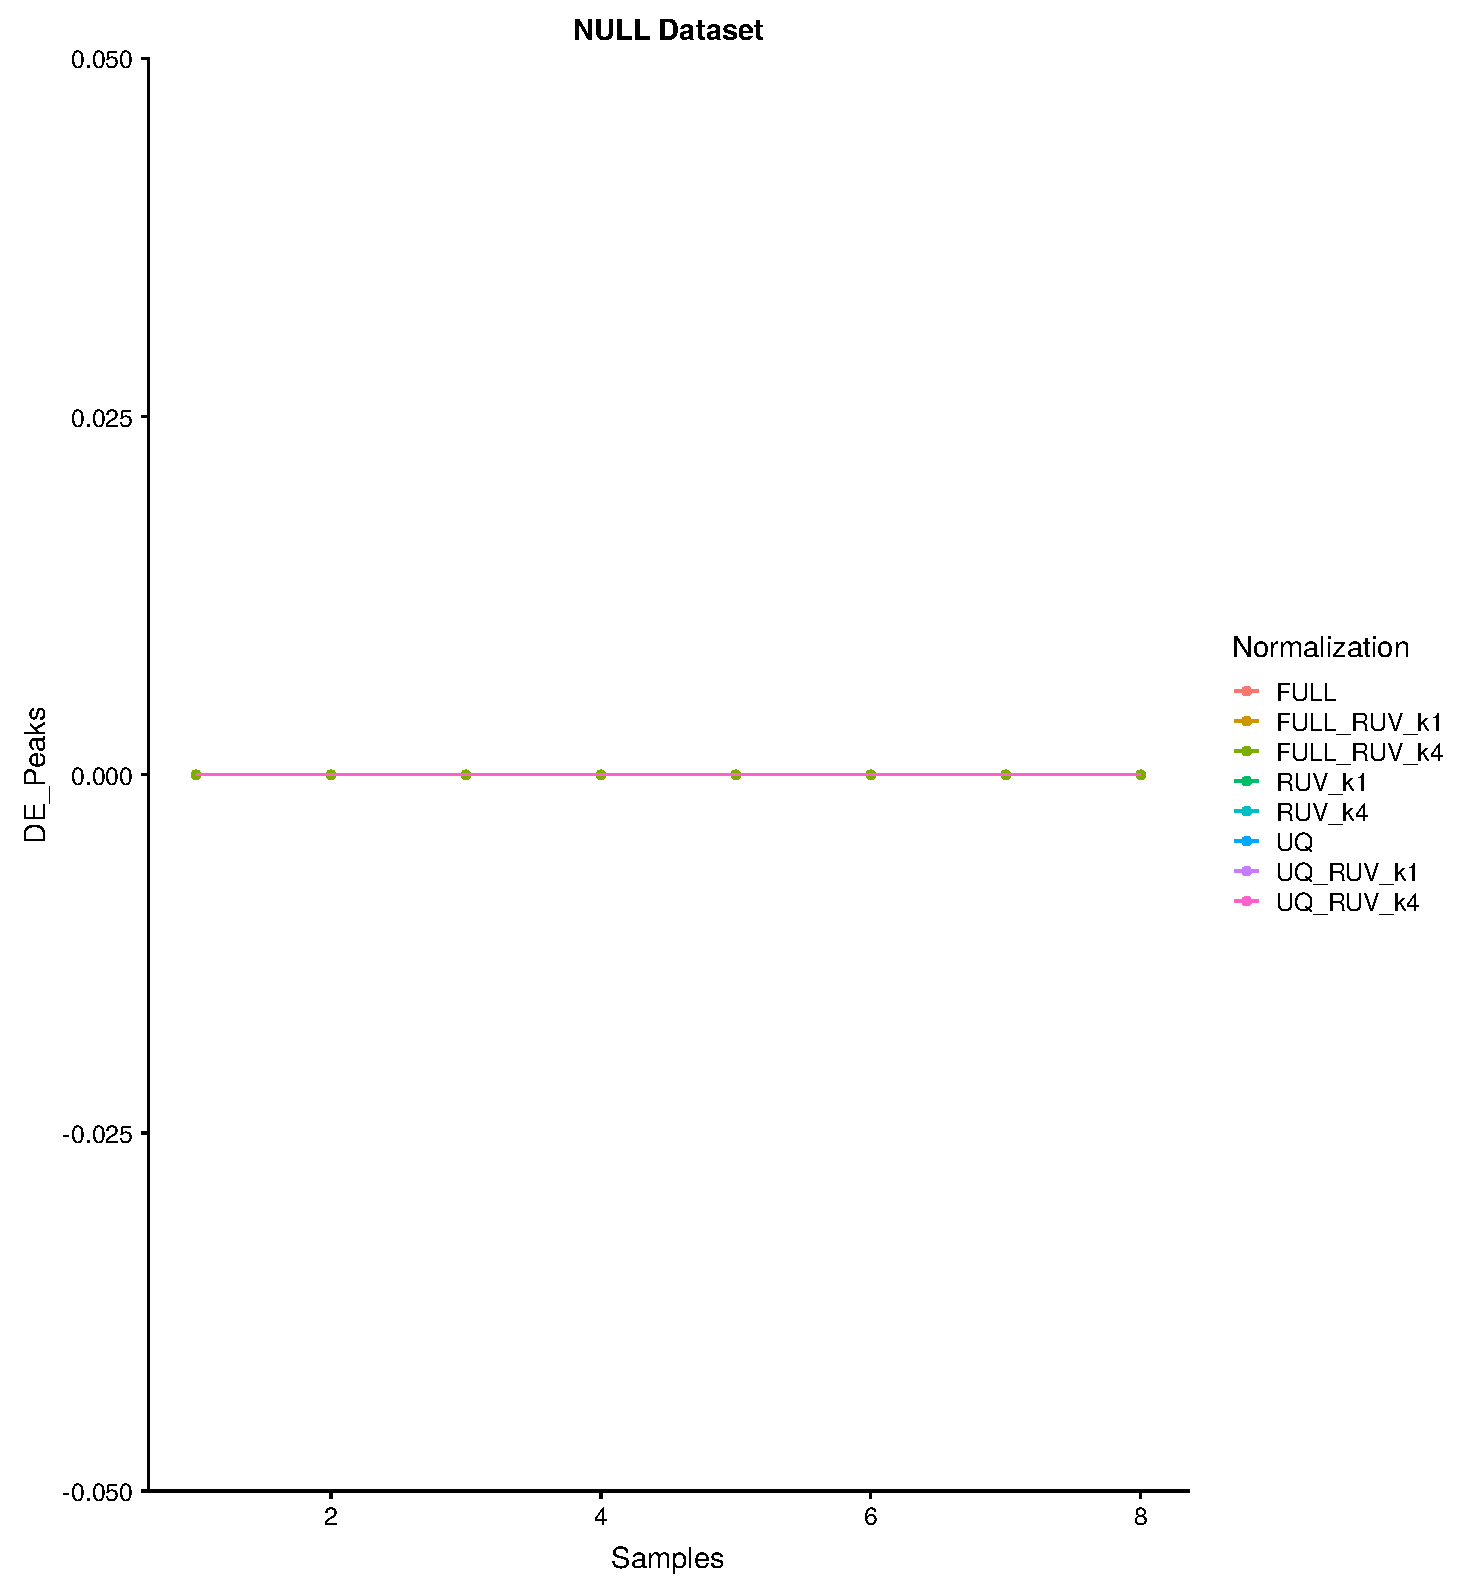
\includegraphics[width=\textwidth, keepaspectratio]{img/descan2/null_dataset_final.pdf}
\caption[Normalizations applied to null dataset]{The figure shows the effects of different normalizations on a null dataset of epigenetic regions, putting in relation the \glspl{der} with the threshold on the samples used to align peaks.}
\label{fig:normalizationsnull}
\centering
\end{figure}

Figure \ref{fig:normalizationsnull} shows, as expected, no \gls{der} detection. 
Highlighting that even if a normalization is applied, once reduced the false positives number, we are confident with our results.


\begin{figure}[H]
\centering
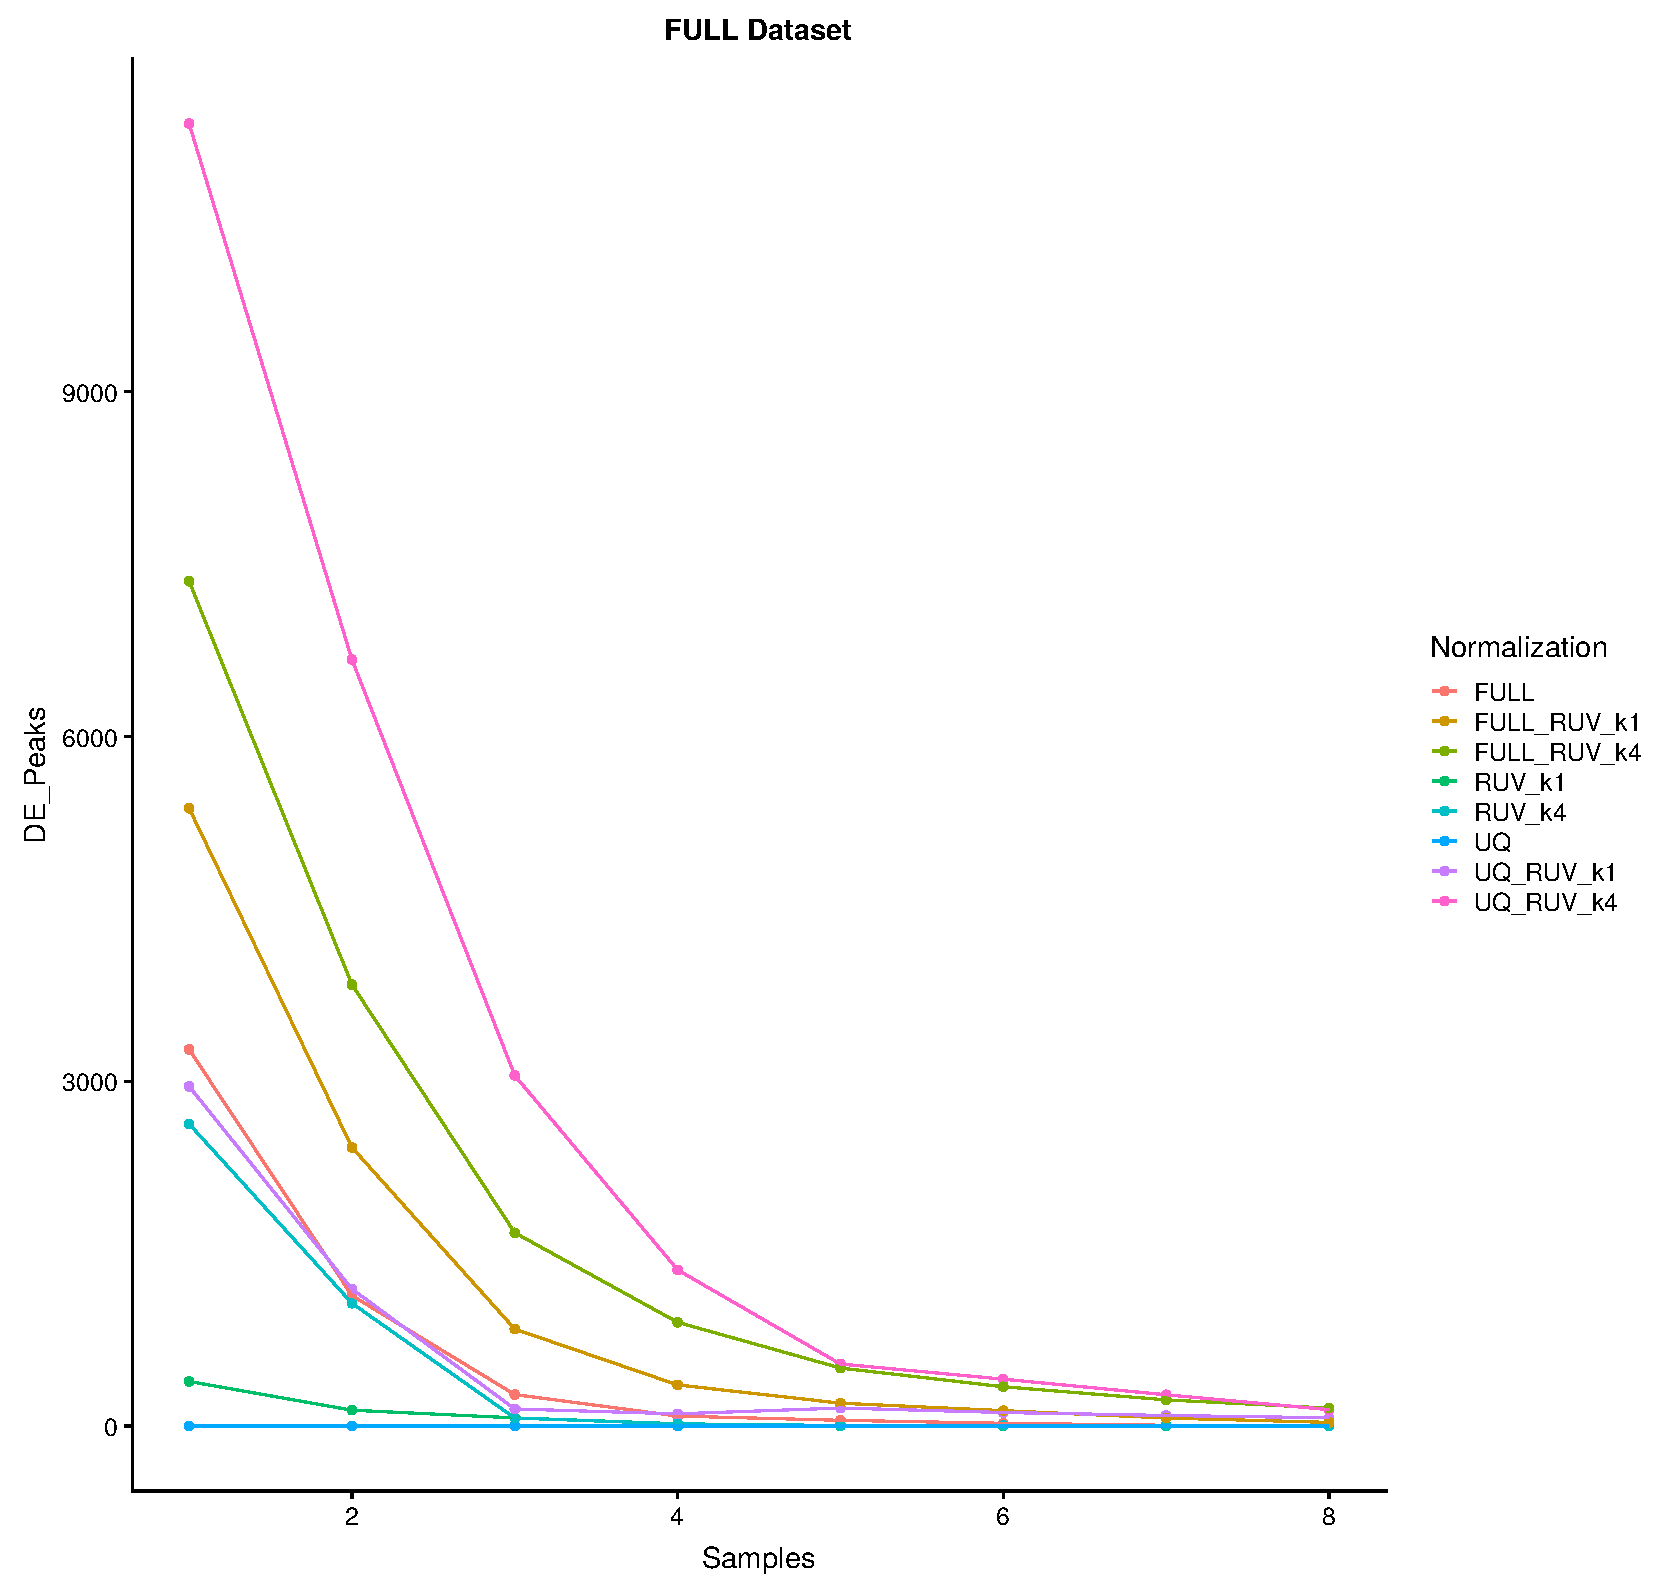
\includegraphics[width=\textwidth, keepaspectratio]{img/descan2/full_final.pdf}
\caption[Normalizations applied to detected regions]{The figure shows the effects of different normalizations on a dataset of epigenetic regions, putting in relation the \glspl{der} with the threshold on the samples used to align peaks.}
\label{fig:normalizationsfull}
\centering
\end{figure}

While figure \ref{fig:normalizationsfull}, representing the "full dataset", shows that \textit{upper-quantile}, by itself is not able to linearly detect any amount of \glspl{der}.
When using \textit{RUVSeq}, the \glspl{der} detection depends on the parameter used (figures \ref{fig:normalizationsnull}, \ref{fig:normalizationsfull} are made using k equal to 1 and 4, for \textit{RUVSeq} normalization).
While, the \textit{full-quantile}, even when used alone is able to detect a good amount of \glspl{der}.
But each normalization, when combined with \textit{RUV-Seq}, seems to affect the data in a way that overestimates the number of \glspl{der}. 
In particular, even the \textit{Upper quartile}, which doesn't detect any signal by itself, is able to detect the highest amount of \glspl{der} when combined with \textit{RUV-Seq}.
%When looking at the \textit{full-quantile} and \textit{RUV-Seq} by themselves seem to perform better than the other normalizations. The first one has a downhill almost linear, while the second one has a very fast downhill with a regrowth when the number of samples is higher.

Even if these normalization methods show good performances with this type of epigenomics data, our investigations suggest that more testing is required, and maybe an ad-hoc normalization method for these data has to be developed.

The left panel represents the "null dataset" highlighting that portion of \glspl{der} due to randomness/bias. Indeed, any kind of normalization produces almost the same trend, underlying that \textit{full quantile}, even if combined with \textit{RUV-Seq} still not reduces the bias.
While \textit{upper quartile} preserves oscillations when using 7/8 samples.
The one which seems to well interpret the data, producing a good compromise between bias and signal, is RUV-Seq.
Indeed, it preserves a gradually downhill of the \gls{der} without totally flatten the signal.

%\begin{figure}[H]
%\centering
%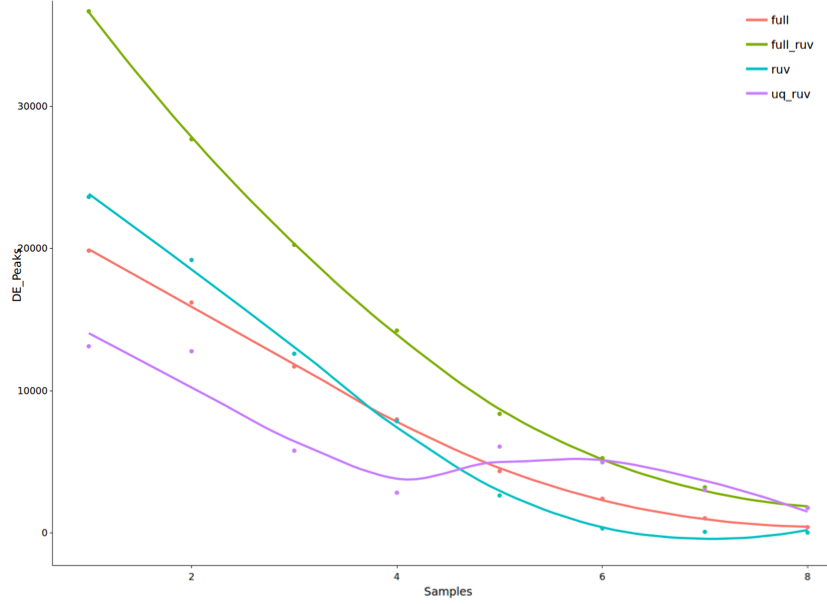
\includegraphics[width=\textwidth, height=\textheight, keepaspectratio]{img/descan2/normalizations.png}
%\caption[Normalizations applied to detected regions]{The figure shows the effects of different normalizations on the epigenomic differentially enriched regions.}
%\label{fig:normalizationsdescan}
%\centering
%\end{figure}
\subsubsection{Differential Enrichment of Peaks}

To estimate the \glspl{der}, any of the RNA-Seq methods can be applied, such as \textit{DESeq2}, \textit{edgeR}, \textit{NOISeq}, etc \cite{Robinson2009, McCarthy2012, Tarazona2011, Tarazona2015}.

\begin{figure}[H]
\centering
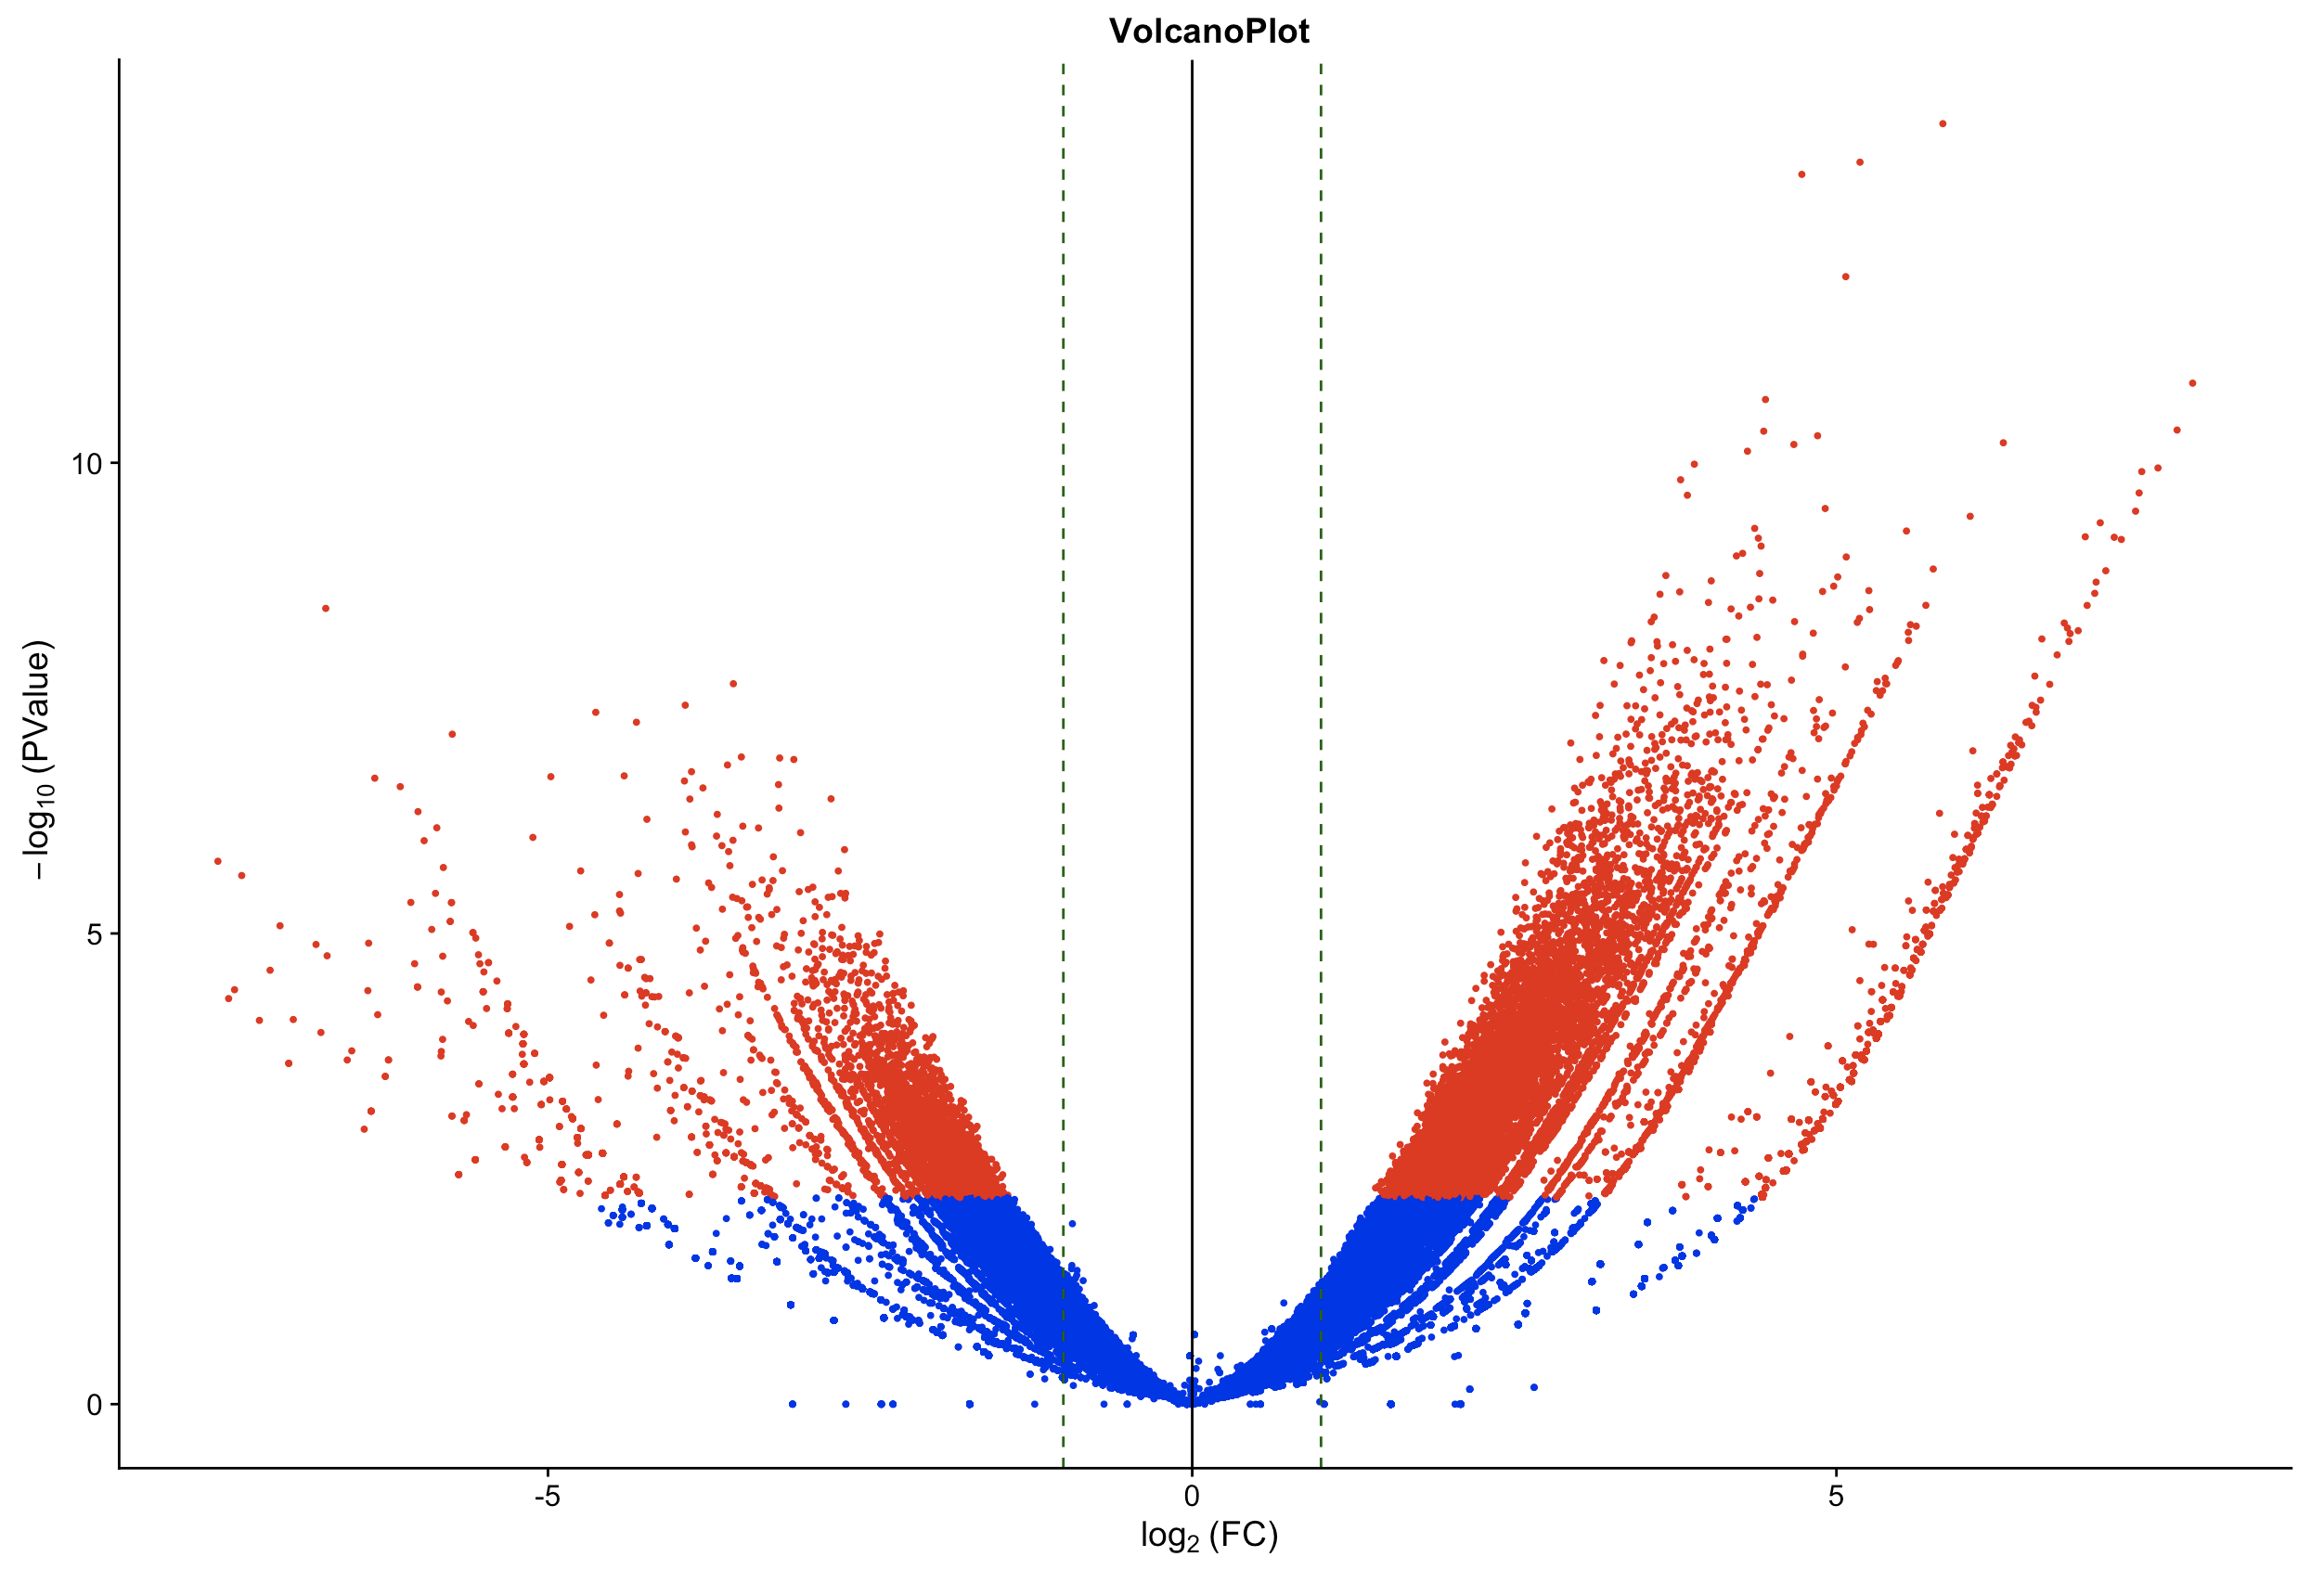
\includegraphics[width=\textwidth, keepaspectratio]{img/descan2/DE_peaks.png}
\caption[Differential Enrichment Regions Volcano]{A volcano plot of Differential Enriched Regions. Blue dots represent the not significant \glspl{der}, while the red ones represent the significant \glspl{der}.}
\label{fig:depeaksdescan}
\centering
\end{figure}

In this case, we decided to use \textit{edgeR} package, because of its wide range of  available statistical approaches and the possibility to better tune the design of the experiment. 
Indeed, because we used the \textit{RUVSeq} normalized counts with \lstinline!k! parameter set to 4, we modelled the experimental design with the \lstinline!model.matrix! function, adding to our model not only the experimental conditions, but also the \textit{RUV-Seq} estimated factors.
Then we used the resulted design to estimate the dispersion and fit a Quasi-Likelihood test, as defined in edgeR\cite{Robinson2009}.
 
\begin{figure}[H]
\centering
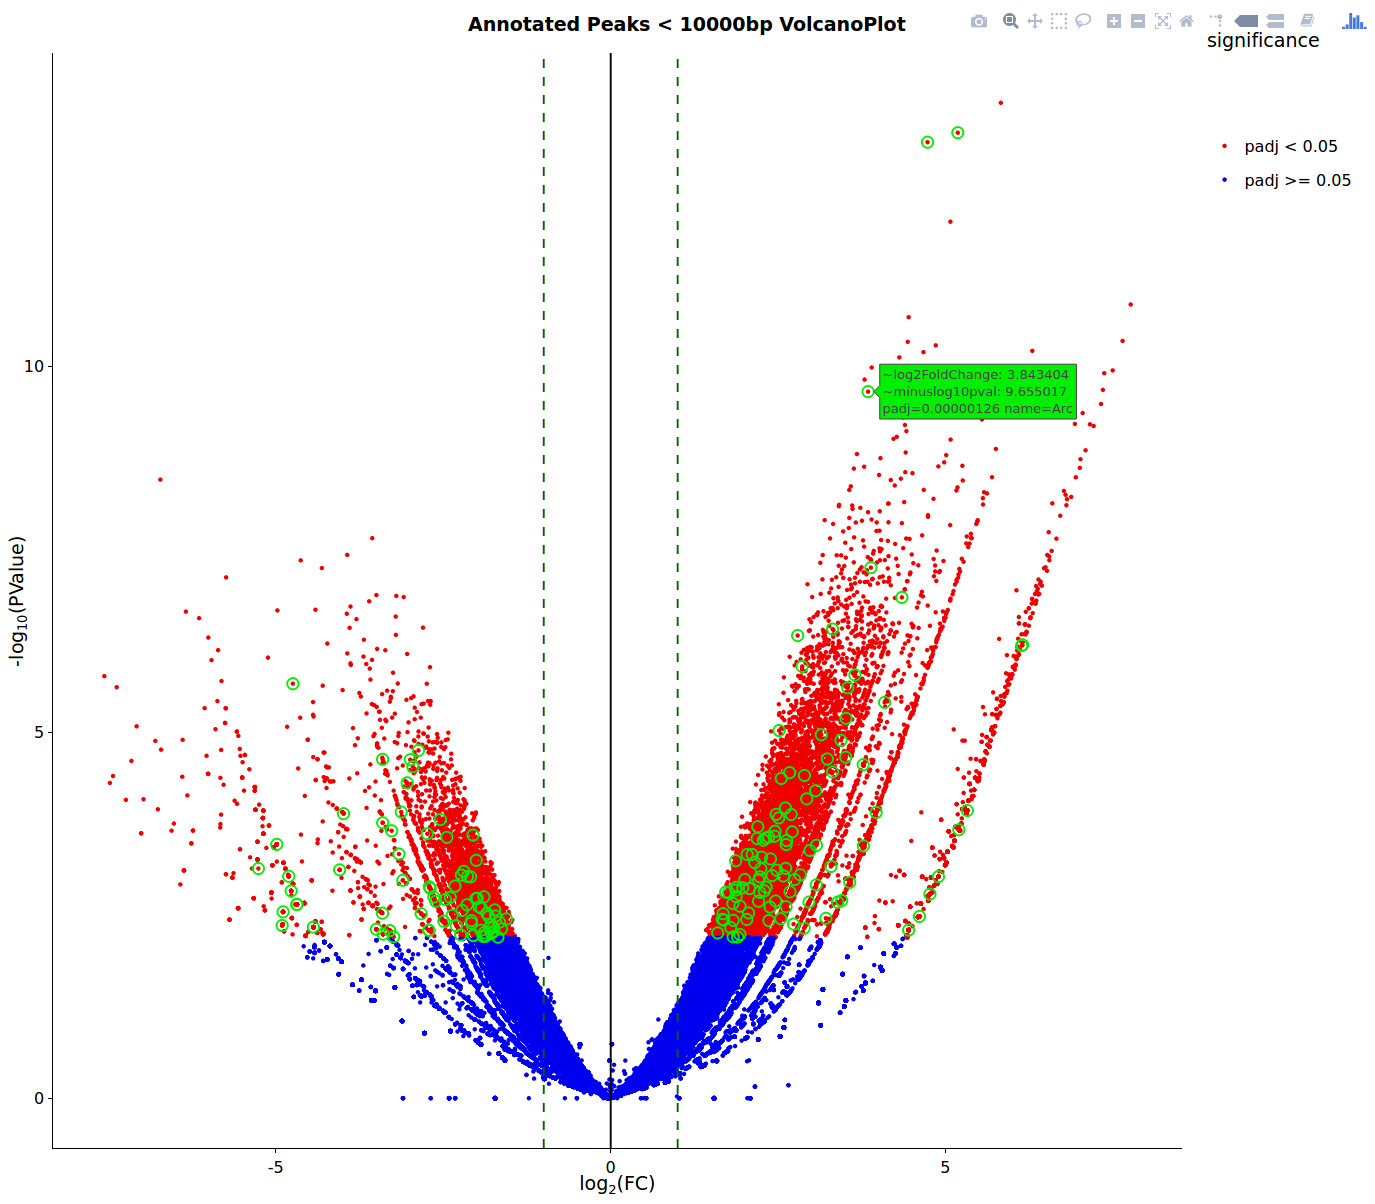
\includegraphics[width=\textwidth, keepaspectratio]{img/descan2/Annotated_depeaks_degenes.png}
\caption[Annotated Differential Enrichment Regions Volcano]{A volcano plot of \glspl{der}. Blue dots represent the not significant \glspl{der}, while the red ones represent the significant \glspl{der}. Green circles highlights the peaks with a \gls{deg} annotated.}
\label{fig:depeakdegenessdescan}
\centering
\end{figure}

Figure \ref{fig:depeaksdescan} shows a volcano plot of \glspl{der} between E0 and E1 conditions.
Red dots highlight the regions with a \gls{fdr}\cite{Benjamini1995} lower than 0.05, while blue dots highlight non significant regions.

\subsubsection{Peaks Integration}

The next task is to integrate the obtained results with other omic data types, as \textit{RNA-seq}. 
Because of the low number of the samples, the easiest way to integrate the data is to annotate the \glspl{der} with \glspl{deg} resulting from the analysis of RNA-Seq.

For the differential expression of the \textit{RNA-seq} data, we first quantified the signal with the \lstinline!featureCounts! methods available in the \textit{Rsubread} \cite{Liao2013} R/Bioconductor package.
Then we filtered lowly expressed genes with the \textit{proportion} test as implemented in \textit{NOISeq} package, and applied the \lstinline!noiseq! method for differential expression.

We used the resulting significant \glspl{deg} (with posterior probability higher than 0.95) to annotate the peaks with \lstinline!annotatePeakInBatch! method of \textit{ChIPpeakAnno}.
Figure 	\ref{fig:depeakdegenessdescan} illustrates with green circles the peaks with an annotated gene with distance lower than 10000bp from the gene \gls{tss}, producing a total of 430 annotated peaks.
Realizing the plot with \textit{ggplot2} combined with \textit{plotly} library it is possible to enhance the names of the genes with a tooltip.

Then, to obtain a seconf level of data integration, we used the annotated genes to do functional annotation on \gls{go} \cite{GeneOntologyConsortium2004, GeneOntologyConsortium2015} and Reactome pathways, which showed several interesting results for the neuronal regulation.

%\textbf{Insert tables for the functional results, to discuss with Davide/Lucia}







